\section*{Introduction}
Exploratory behavior can have two very different explanations depending on the expected result. If rewards are expected, then exploration is cast as a search for reward \cite{Gupta2006,Sutton2018,Woodgate2017,Lee2011a,Schulz2018a,Calhoun2014}. This is how exploration is commonly framed \cite{Sutton2018}. If instead there is no reason to expect rewards, exploration is cast as a search for information, novelty, or curiosity \cite{Berlyne1950,Schmidhuber1991,Kidd2015,Jaegle2019,Sumner2019,Wang2019,Auersperg2015}. For example, a rat placed in a novel maze will explore, extensively, even when no rewards could be expected \cite{Rosenberg2021}.

An open problem in decision science is to unify exploration--of any kind--with exploitation, often defined by taking most rewarding action. When exploration optimizes for reward, which is the the classic view, this union leads to the famous exploration-exploitation dilemma \cite{Kelly1956,Berger-Tal2014,Dayan1996,Thrun1992,Mehlhorn2015,Kobayashi2019}, which we illustrate in Fig. \ref{fig:bee}a. In this paper, we offer an alternative approach. We unify exploitation with curiosity instead, which we illustrate in Fig. \ref{fig:bee}b.  

It is easy to justify our use of curiosity, in this way. Curiosity is a primary drive \cite{Berlyne1950,Loewenstein1994,Inglis2001}. It is a drive that is as strong as the drive for reward, if not stronger \cite{Loewenstein1994,Kidd2015,Gottlieb2018,Sumner2019,Gopnik2020,Song2019,Wang2019}. Curiosity is highly effective at solving difficult optimization problems, both in the long-term and the short-term \cite{Schmidhuber1991,Pathak2017,Stanton2018,Fister2019,Mouret2015,Colas2020,Cully2015,Pathak2017,Schwartenbeck2019,Laversanne-Finot2018}. 

We will first develop the theory behind our union. This consists of mathematical study of curiosity alone, then with reward collection. The second half presents initial simulations where we compare to, and often exceed, more standard approaches. We conclude with some questions and answers about our approach.

\begin{figure}
	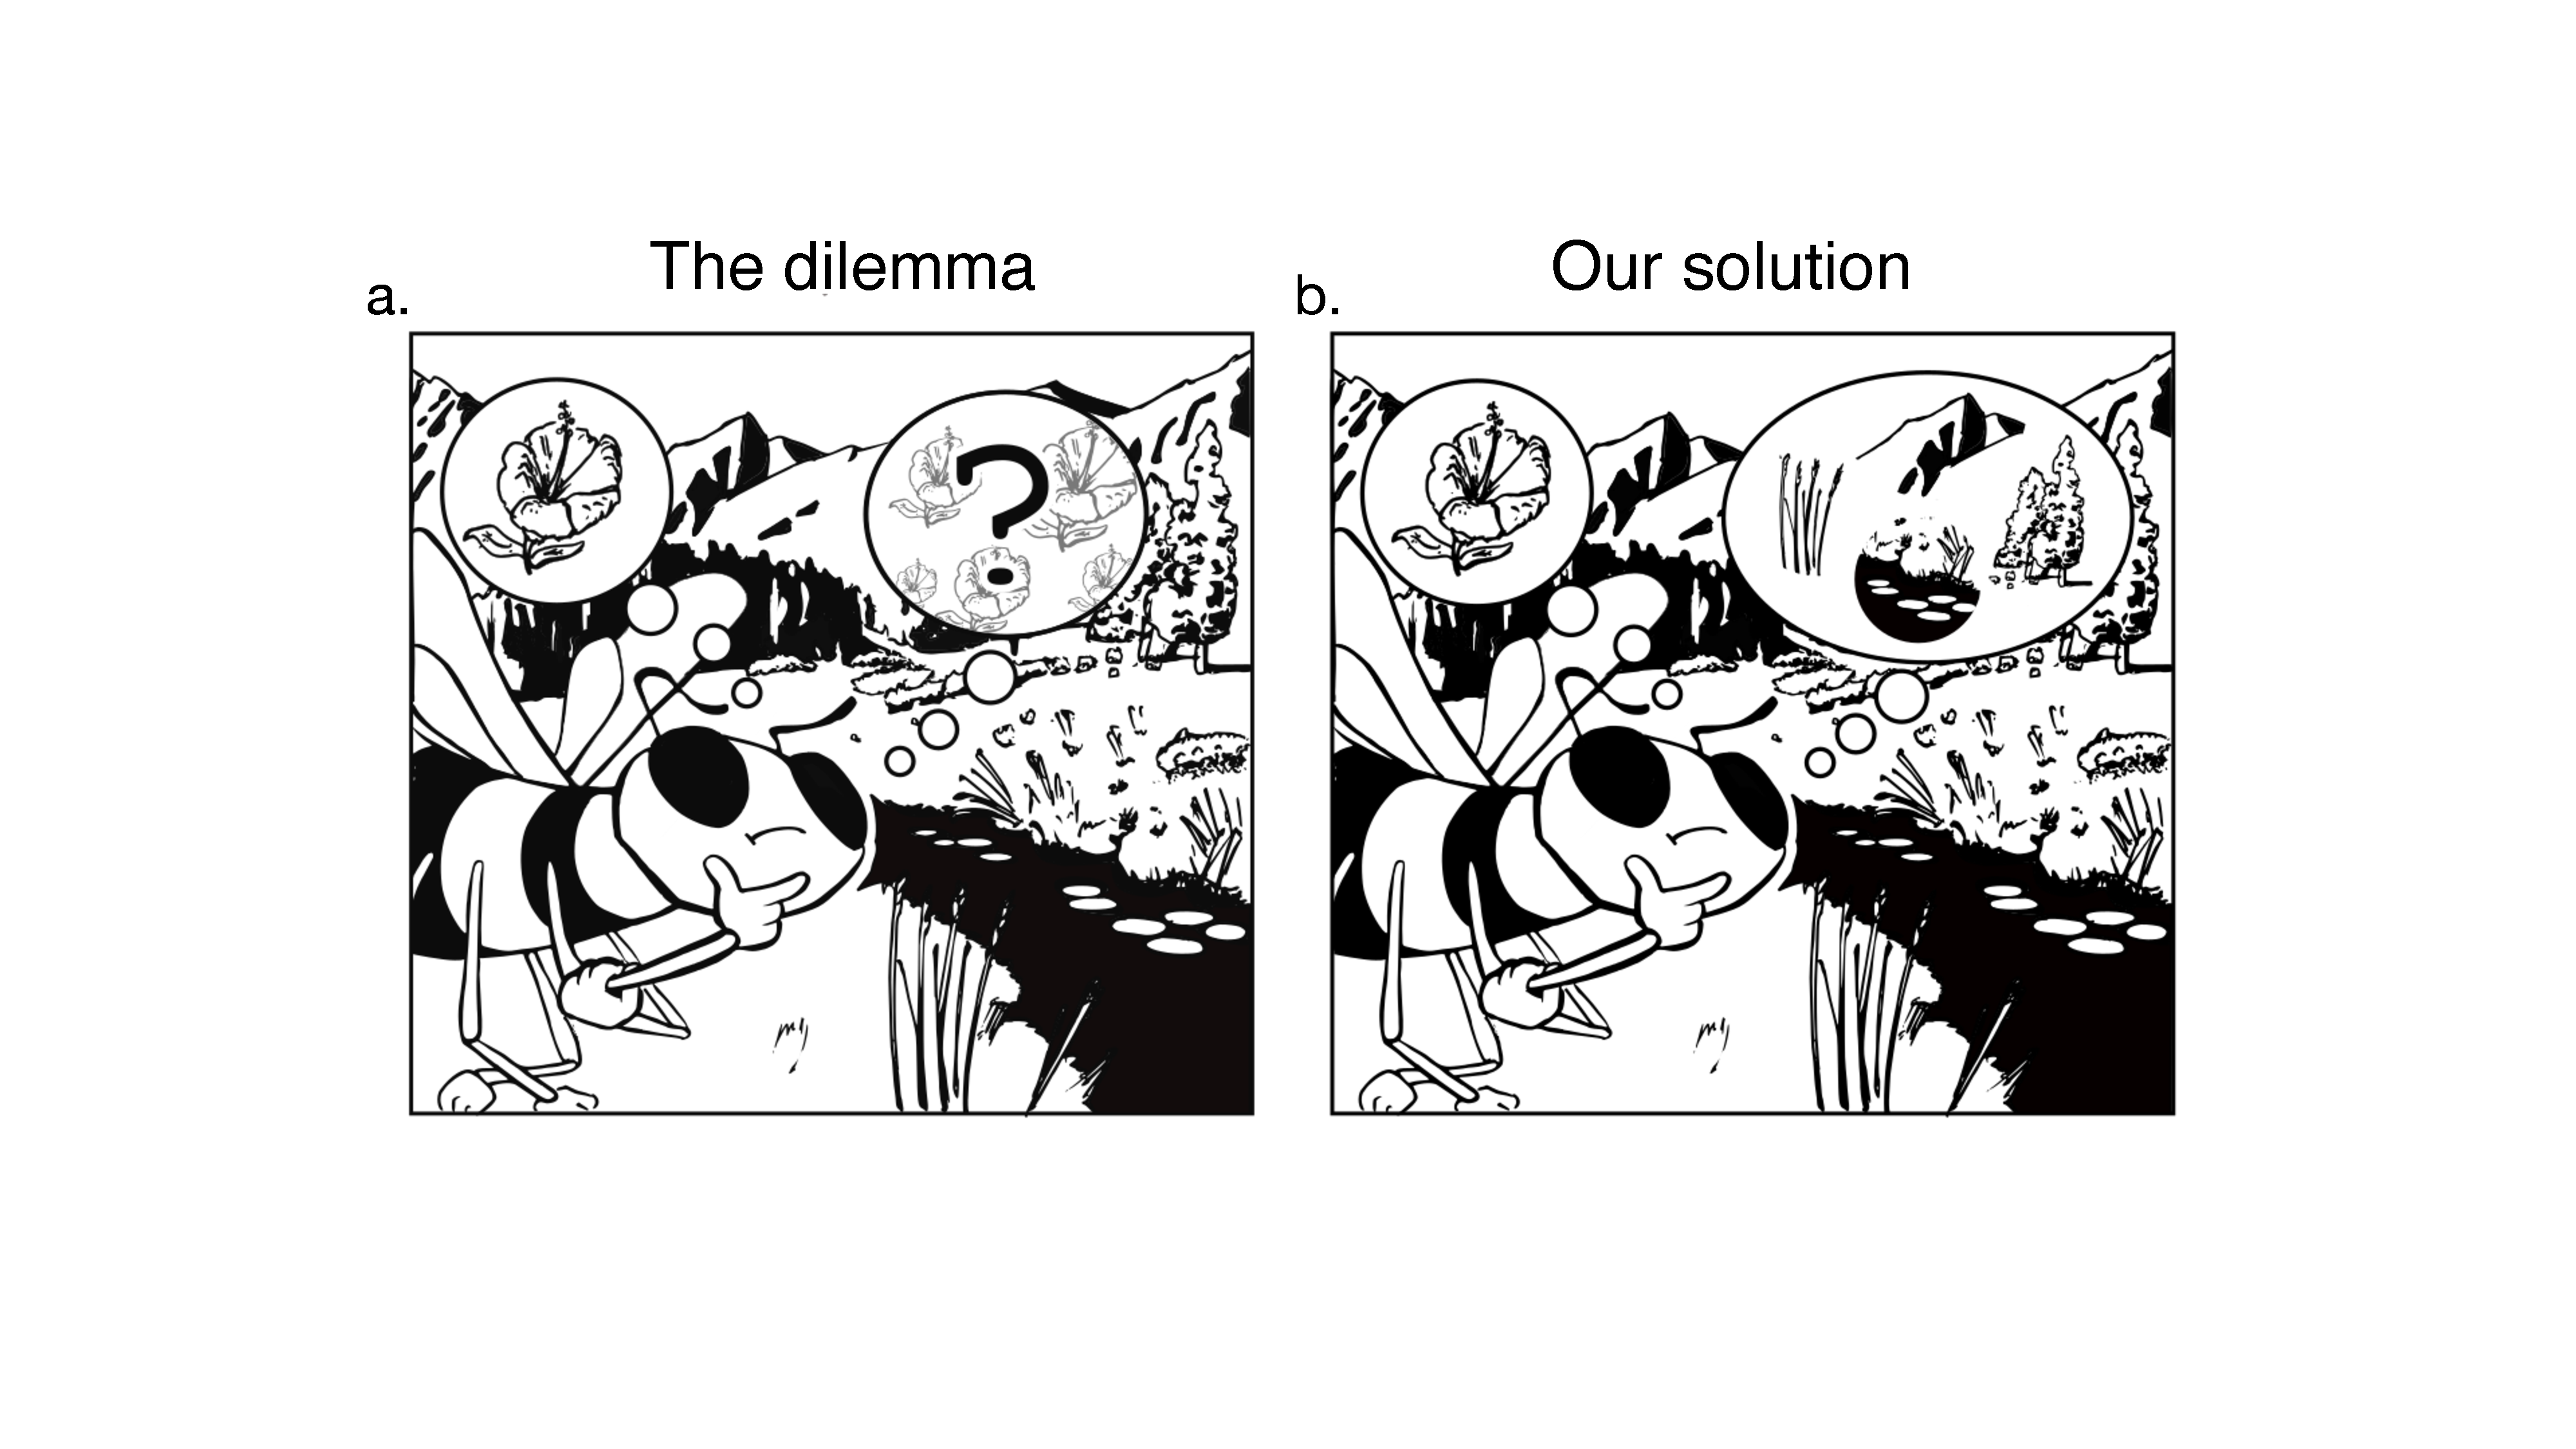
\includegraphics[width=.9\linewidth]{img/bee.pdf} 
	\caption{Two views of exploration and exploitation. \textbf{a}. The dilemma: either exploit an action with a known reward (e.g., return to the previous flower) or explore other actions on the chance they will return a better outcome. The central challenge here is that the outcome of exploration is uncertain, and filled with questions. \textbf{b}. Our alternative view of the dilemma, with two goals: either exploit rewards \textit{or} explore to maximize information value, with a curious search of the environment. \textit{Artist credit}: Richard Grant.}
	\label{fig:bee} 
\end{figure}
